\documentclass{beamer}
\usepackage[utf8]{inputenc}
\usepackage[T1]{fontenc}
\usepackage{helvet}
%if you present in German, you have to swap these values
\usepackage[ngerman,english]{babel}

%cool smartdiagrams
\usepackage{smartdiagram}
\usesmartdiagramlibrary{additions}

%for mathfont
\usefonttheme[onlymath]{serif}

%colortheme
\usecolortheme{tum}
\useoutertheme[footline=authortitle,subsection=false]{miniframes}

%font
\setbeamerfont{author}{size=\footnotesize}
\setbeamerfont{date}{size=\scriptsize}

%for itemize
\usepackage{enumitem}
\setitemize{label=\usebeamerfont*{itemize item}%
  \usebeamercolor[fg]{itemize item}
  \usebeamertemplate{itemize item}}
\setlist[itemize,1]{leftmargin=2em}
\useinnertheme{rectangles}

\usepackage{pgf}  
\usepackage{tikz}

\setbeamertemplate{frametitle}
{
  \nointerlineskip
  \begin{beamercolorbox}[sep=0.3cm,rightskip=2cm,wd=\paperwidth]{frametitle}
      \usebeamerfont{frametitle}
      \vbox{}\vskip-1ex
      \strut\insertframetitle\strut
      \hfill
      \vskip-0.8ex
  \end{beamercolorbox}
}
\addtobeamertemplate{frametitle}{}{
  \begin{tikzpicture}[remember picture,overlay]
  \node[anchor=north east,yshift=-0.45cm] at (current page.north east) {
\includegraphics[width=0.35\textwidth]{figures/TH-Nuernberg-RGB.png}};
  \end{tikzpicture}
}

%for the logo in the upper right corner
\usepackage{textpos}

 
\titlegraphic{
\begin{beamercolorbox}[wd=\paperwidth,dp=1ex, ht=5.5ex, sep=1.5ex, colsep*=0pt]{frametitle}%
    \usebeamerfont{frametitle}   \strut \insertframetitle  \hfill  \raisebox{-1.5ex}[0pt][-\ht\strutbox ]{ 
\includegraphics[width=0.35\textwidth]{figures/TH-Nuernberg-RGB.png}}
    \end{beamercolorbox}%
 }


\setbeamertemplate{title page}
{
  \usebeamercolor[fg]{titlegraphic}\inserttitlegraphic\par
	\vbox{}
	\vfill
	\begin{flushleft}
		\begin{beamercolorbox}[sep=8pt,left]{title}
			\usebeamerfont{title}\inserttitle\par%
			\ifx\insertsubtitle\@empty%
			\else%
				\vskip0.25em%
				{\usebeamerfont{subtitle}\usebeamercolor[fg]{subtitle}\insertsubtitle\par}%
			\fi%
    	\end{beamercolorbox}%
    	\vskip1em\par
		\begin{beamercolorbox}[sep=8pt,left]{author}
		\usebeamerfont{author}\insertauthor
		\end{beamercolorbox}
		\begin{beamercolorbox}[sep=8pt,left]{institute}
		\usebeamerfont{institute}\insertinstitute
		\end{beamercolorbox}
		\begin{beamercolorbox}[sep=8pt,left]{date}
		\usebeamerfont{date}\insertdate
		\end{beamercolorbox}\vskip0.5em
		
	\end{flushleft}
	\vfill
}

\mode<presentation>

\title[Your Super Fancy Title]{Your Super Fancy Title}
\subtitle{Bachelorthesis in Computer Science}

\author{Your Name}
\institute[]{Fakultät Informatik}
\date{21th February 2020}


%fuer fancy overlay graphics
\def\Put(#1,#2)#3{\leavevmode\makebox(0,0){\put(#1,#2){#3}}}

%fuer tables mit bildern
\usepackage{tabularx}
\usepackage{caption}
\setbeamerfont{caption}{size=\scriptsize}
\captionsetup{justification=centering}

%%for table input
\usepackage{booktabs}
\usepackage{adjustbox}
%%

% mindblowing things happen
% itemize items on the same height
\newcommand\parallelcontent[2]{
  \begin{columns}[t]
    \column{0.5\textwidth} #1
    \column{0.5\textwidth} #2
  \end{columns}
}
\newcommand\parallelitem[2]{
  \parallelcontent
  {\begin{itemize} \item #1 \end{itemize}}
  {\begin{itemize} \item #2 \end{itemize}}
}

%font size caption
\setbeamerfont{caption}{series=\tiny,size=\fontsize{14}{16}} 



\begin{document}

\begin{frame}
\titlepage
\end{frame}

\begin{frame}[c]{}
\centering
\vspace{-3em}
\frametitle{Contents}
 \smartdiagramset{
 planet size=2cm,
 planet text width=3cm,
 planet font=\large,
 satellite size=1.8cm, 
 satellite text width=2cm,
 satellite font=\normalsize,
 distance planet-text=0,
 distance planet-satellite=3.5cm,
 /tikz/connection planet satellite/.append style={<-},
 set color list={red!40 , cyan!40 , blue!40 , green!40 , orange!60 , yellow!60 , magenta!40 , brown!40 , violet!40}
 } 

\begin{center}
\scalebox{0.75}{
\smartdiagramset{planet color=orange!60}
\smartdiagramanimated[connected constellation diagram]
{Center,
One,
Two,
Three,
Four,
Five,
Awesome
}
}
\end{center}
\end{frame}

\begin{frame}[t]
\frametitle{Daten}
Classical Itemize
\begin{itemize}
	\item Item1
	\item Item2
	\begin{itemize}
		\item Item2.1
		\item Item2.2 and cite something for fun \cite{Goodliffe2007}
	\end{itemize}
	\item Item3
\end{itemize}
\end{frame}

\begin{frame}[t]
\frametitle{Cool Function}
Pearson Correlation Coefficient
%
\begin{align}
r _ { x y }  = \frac { \sum\limits _ { i = 1 } ^ { n } ( x _ { i } - \overline { x } ) ( y _ { i } - \overline { y } ) } { \sqrt { \sum\limits _ { i = 1 } ^ { n } ( x _ { i } - \overline { x } ) ^ { 2 } \cdot \sum\limits _ { i = 1 } ^ { n } ( y _ { i } - \overline { y } ) ^ { 2 } } } 
\end{align}
%
\end{frame}

\begin{frame}[t]{}
\frametitle{Your toooooooo \\looooooong Title}
 \begin{center}
 \vspace{-2em}
 \scalebox{0.8}{
\smartdiagramset{planet color=orange!60}
\smartdiagramanimated[bubble diagram]
{ Center,
Something\\Cool, 
Another\\Fact, 
Last Fact
}}
\end{center}
\end{frame}

\begin{frame}[t]
\frametitle{Seperate Images \\Side by Side}
 \vspace{-2em}
\begin{center}
\begin{tabularx}{\columnwidth}{>{\centering\arraybackslash}X>{\centering\arraybackslash}X}
       \large Macro Location &     \large Mikro Location \\ 
       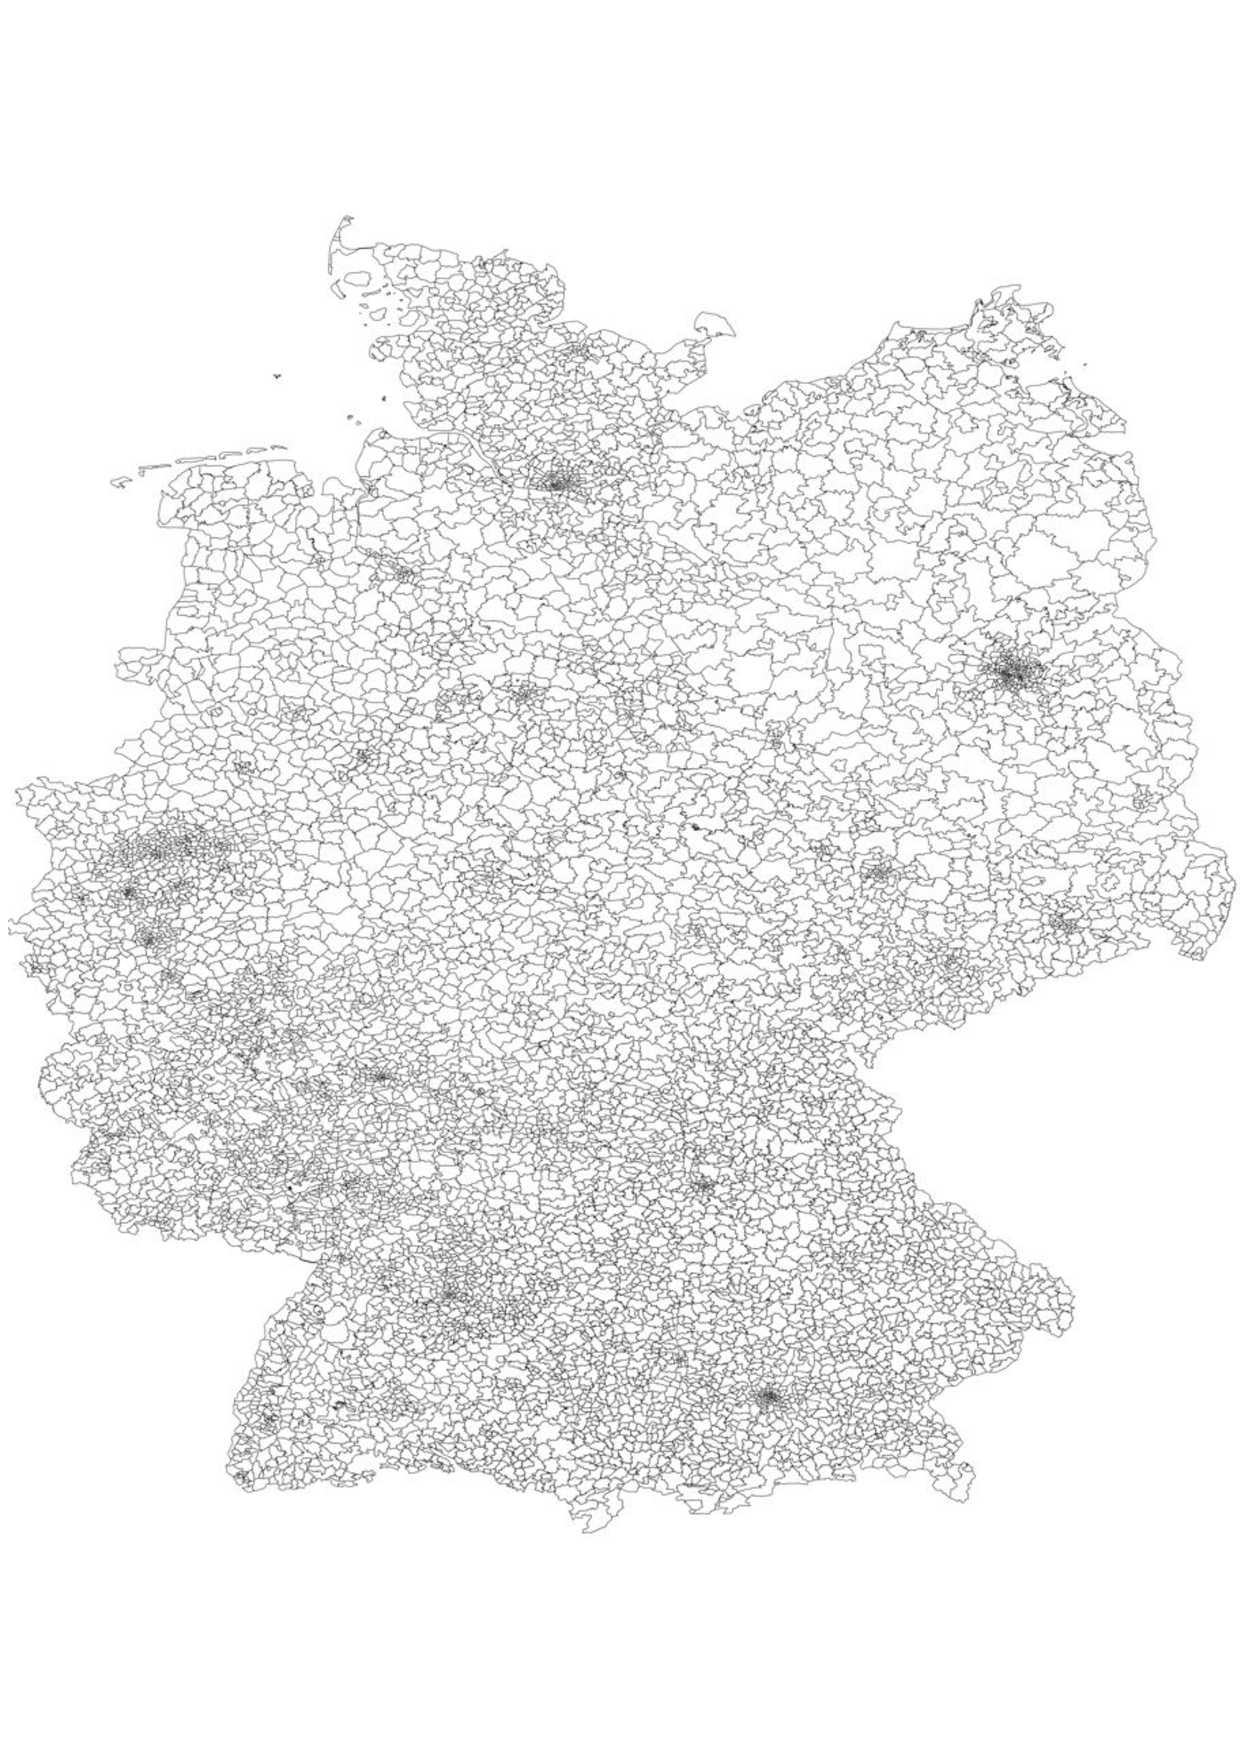
\includegraphics[width=0.4\textwidth]{figures/zip_ger_compr} \captionof{figure}{ Figure 1}
       &
       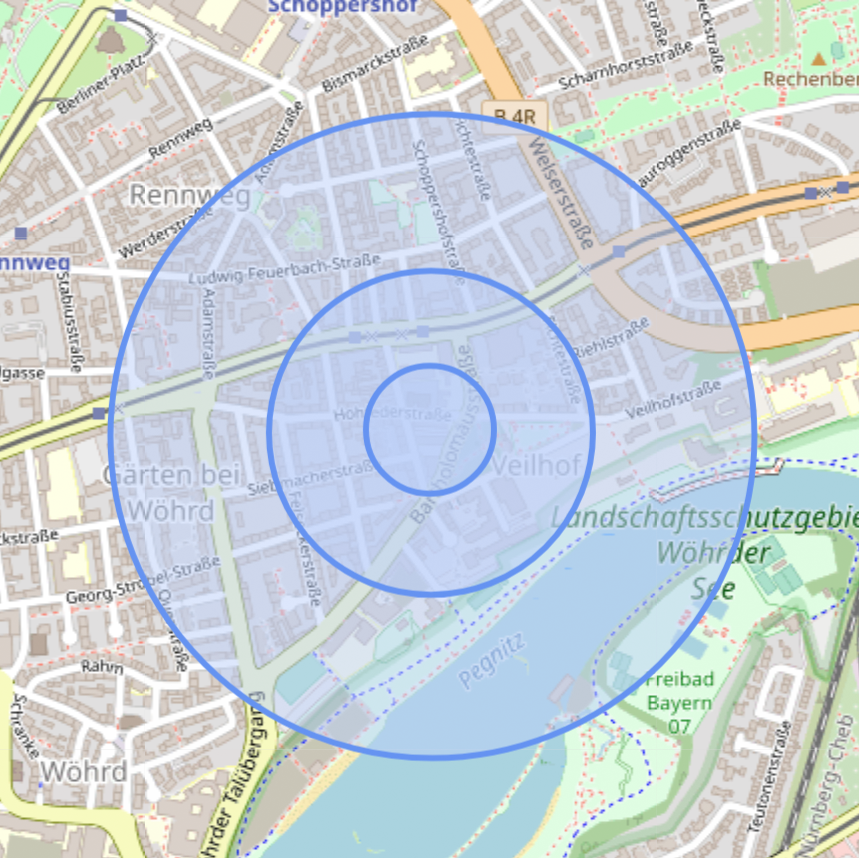
\includegraphics[width=0.4\textwidth]{figures/three_radii_fig_poster_v2}\captionof{figure}{Figure 2} \\ 
\end{tabularx}
\end{center}
\end{frame}

\begin{frame}[t]
\frametitle{Side by Side Iteration}
\small
\centering
\parallelcontent
  {Cool Stuff}
  {Fancy Stuff}
  \parallelitem
  {Very long long long long long long long long long long long long long long long long text}
  {Short text}
  \parallelitem
  {Stuff}
  {Other stuff}
  \parallelitem
  {Another stuff}
  {Other another stuff}
\end{frame}

\begin{frame}[allowframebreaks, t]
\frametitle{Bibliography}
\vspace{-1.9em}
\tiny
%bib
\setbeamertemplate{bibliography item}[text]
\bibliographystyle{wmaainf}
\bibliography{refs}
\end{frame}

\begin{frame}[c]
\frametitle{~}
 \vspace{-1.9em}
\hfill
    \begin{beamercolorbox}[center, wd=10cm]{title}
        \huge Questions?
    \end{beamercolorbox}
\hfill\hfill
\end{frame}

\setbeamercolor{background canvas}{bg=black}
\setbeamertemplate{navigation symbols}{}
\begin{frame}[plain]{}

\end{frame}

\end{document}
